%%%%%%%%%%%%%%%%%%%%%%%%%%%%%%%%%%%%%%%%%%%%%%%%%%%%%%%%%%%%%%%%%%%%%%%%%%%%%%%%%%%%%%%%%%%%%%%%%%%%%%
% Plantilla básica de Latex en Español.
%
% Autor: Andrés Herrera Poyatos (https://github.com/andreshp) 
%
% Es una plantilla básica para redactar documentos. Utiliza el paquete fancyhdr para darle un
% estilo moderno pero serio.
%
% La plantilla se encuentra adaptada al español.
%
%%%%%%%%%%%%%%%%%%%%%%%%%%%%%%%%%%%%%%%%%%%%%%%%%%%%%%%%%%%%%%%%%%%%%%%%%%%%%%%%%%%%%%%%%%%%%%%%%%%%%%

%-----------------------------------------------------------------------------------------------------
%	INCLUSIÓN DE PAQUETES BÁSICOS
%-----------------------------------------------------------------------------------------------------

\documentclass[10pt]{article}

%-----------------------------------------------------------------------------------------------------
%	SELECCIÓN DEL LENGUAJE
%-----------------------------------------------------------------------------------------------------

% Paquetes para adaptar Látex al Español:
\usepackage[spanish,es-noquoting, es-tabla, es-lcroman]{babel} % Cambia 
\usepackage[utf8]{inputenc}                                    % Permite los acentos.
\selectlanguage{spanish}                                       % Selecciono como lenguaje el Español.

%-----------------------------------------------------------------------------------------------------
%	SELECCIÓN DE LA FUENTE
%-----------------------------------------------------------------------------------------------------

% Fuente utilizada.
\usepackage{microtype}                  % Mejora la letra final de cara al lector.
\usepackage{helvet}

\renewcommand{\familydefault}{\sfdefault}

%-----------------------------------------------------------------------------------------------------
%	ESTILO DE PÁGINA
%-----------------------------------------------------------------------------------------------------

% Paquetes para el diseño de página:
\usepackage{fancyhdr}               % Utilizado para hacer títulos propios.
\usepackage{lastpage}               % Referencia a la última página. Utilizado para el pie de página.
\usepackage{extramarks}             % Marcas extras. Utilizado en pie de página y cabecera.
\usepackage[parfill]{parskip}       % Crea una nueva línea entre párrafos.
\usepackage{geometry}               % Asigna la "geometría" de las páginas.

% Se elige el estilo fancy y márgenes de 3 centímetros.
\pagestyle{fancy}
\geometry{left=3cm,right=3cm,top=2.5cm,bottom=2.5cm,headheight=1cm,headsep=0.5cm} % Márgenes y cabecera.
% Se limpia la cabecera y el pie de página para poder rehacerlos luego.
\fancyhf{}

% Espacios en el documento:
\linespread{1}                        % Espacio entre líneas.
\setlength\parindent{0pt}               % Selecciona la indentación para cada inicio de párrafo.

% Cabecera del documento. Se ajusta la línea de la cabecera.
\renewcommand\headrule{
	\begin{minipage}{1\textwidth}
	    \hrule width \hsize 
	\end{minipage}
}

% Texto de la cabecera:
\lhead{\subject}               % Parte izquierda.
\chead{}                       % Centro.
\rhead{\doctitle}              % Parte derecha.

% Pie de página del documento. Se ajusta la línea del pie de página.
\renewcommand\footrule{                                 
\begin{minipage}{1\textwidth}
    \hrule width \hsize   
\end{minipage}\par
}

\lfoot{}                                                 % Parte izquierda.
\cfoot{}                                                 % Centro.
\rfoot{Página\ \thepage\ de\ \protect\pageref{LastPage}} % Parte derecha.

%-----------------------------------------------------------------------------------------------------
%	IMÁGENES
%-----------------------------------------------------------------------------------------------------

\usepackage{graphicx}                  % Utilizado para insertar gráficos.
\usepackage{caption}                   % Títulos y leyendas para los gráficos.
\usepackage{subcaption}                % Subfiguras.
\usepackage{float}

%-----------------------------------------------------------------------------------------------------
%	BIBLIOGRAFÍA
%-----------------------------------------------------------------------------------------------------

\usepackage[backend=bibtex]{biblatex}
\usepackage{csquotes}

\addbibresource{references.bib}

%-----------------------------------------------------------------------------------------------------
%	ALGORITMOS
%-----------------------------------------------------------------------------------------------------

\usepackage{algorithm}
\usepackage{algorithmic}

%-----------------------------------------------------------------------------------------------------
%	PORTADA
%-----------------------------------------------------------------------------------------------------

% Elija uno de los siguientes formatos.
% No olvide incluir los archivos .sty asociados en el directorio del documento.
\usepackage{title1}
%\usepackage{title2}
%\usepackage{title3}

%-----------------------------------------------------------------------------------------------------
%	TÍTULO, AUTOR Y OTROS DATOS DEL DOCUMENTO
%-----------------------------------------------------------------------------------------------------

% Título del documento.
\newcommand{\doctitle}{Big Data y TPCx-HS}
% Subtítulo.
\newcommand{\docsubtitle}{}
% Fecha.
\newcommand{\docdate}{28 \ de \ Marzo \ de \ 2015}
% Asignatura.
\newcommand{\subject}{Ingeniería de Servidores}
% Autor.
\newcommand{\docauthor}{}
\newcommand{\docaddress}{}
\newcommand{\docemail}{}

%-----------------------------------------------------------------------------------------------------
%	RESUMEN
%-----------------------------------------------------------------------------------------------------

% Resumen del documento. Va en la portada.
% Puedes también dejarlo vacío, en cuyo caso no aparece en la portada.
%\newcommand{\docabstract}{}
\newcommand{\docabstract}{En este texto puedes incluir un resumen del documento. Este informa al lector sobre el contenido del texto, indicando el objetivo del mismo y qué se puede aprender de él.}

\begin{document}

\makeatletter\renewcommand{\ALG@name}{Algoritmo}

\maketitle

%-----------------------------------------------------------------------------------------------------
%	ÍNDICE
%-----------------------------------------------------------------------------------------------------

% Profundidad del Índice:
%\setcounter{tocdepth}{1}

\newpage
\tableofcontents
\newpage

%-----------------------------------------------------------------------------------------------------
%	SECCIÓN 1: INTRODUCCIÓN
%-----------------------------------------------------------------------------------------------------

\section{Introducción} \label{sec:introduction}

	Desde hace miles de años el ser humano ha investigado la manera de almacenar y recopilar información. Durante muchos siglos la escritura y la pintura eran los únicos mecanismos existentes. Posteriormente surgió la fotografía, los discos de vinilo... Sin embargo, poca información seguía ocupando mucho volumen físico. Gracias a los avances tecnológicos de las últimos décadas, hoy en día disponemos dispositivos electrónicos para el almacenamiento de datos binarios. Además, la evolución de estos dispositivos ha sido frenética. IBM comercializó el primer disco duro en 1956. Este constaba solamente de 5 mega bytes de capacidad \cite{hard-disks} mientras que actualmente podemos utilizar discos duros con más de 1 tera byte.

	La capacidad de cómputo y procesamiento de los computadores también ha crecido de forma exponencial. El primer ordenador comercial se presentó en 1951 y se conoce como  UNIVAC 1 \cite{first-commercial-computer}. Este computador tenía una frecuencia de 2.25 mega hercios y 1000 palabras de memoria principal o RAM \cite{caract}. Actualmente utilizamos procesadores con más de 2 giga hercios de frecuencia de reloj. Además, es habitual encontrar computadores con 8 o más giga bytes de memoria principal, lo que permite trabajar con bastante información de forma eficiente. 

	Estas nuevas tecnologías han posibilitado que el almacenamiento de datos sea mucho más sencillo. Podemos guardar multitud de archivos en un dispositivo de unos centímetros y compartirlos con cualquier usuario. Además, el procesamiento de estos archivos a nivel de usuario es eficiente gracias a la velocidad de los computadores. 
	
	El mayor flujo de datos es producido en Internet. Aunque es relativamente joven, se hizo público en 1993, actualmente existen más de mil millones de páginas webs \cite{internet}. Además, multitud de dispositivos electrónicos se conectan e interaccionan con Internet (lo que se denomina Internet de las cosas \cite{big-data-internet-cosas}). Los usuarios de estos dispositivos utilizan aplicaciones web y redes sociales, publicando textos y archivos multimedia. 
	
	Todo este cúmulo de tecnologías y actividades ha dado lugar a que hoy en día haya más de 10 zeta bytes de información almacenados (1 ZB = $10^{12}$ GB). La Figura \ref{fig:zeta-bytes} muestra la evolución histórica de la cantidad de información acumulada por el ser humano. Podemos observar que cada año se generan varios zeta bytes de información, el crecimiento es exponencial. Hasta 2003 se habían almacenado en total 5 exa bytes de información (1 EB = $10^9$ GB). Actualmente, generamos esta cantidad de datos en dos días \cite{big-data}. Podemos decir que vivimos en una sociedad digital o sociedad de la información.

	\begin{figure}[H]
	       	\centering
	       	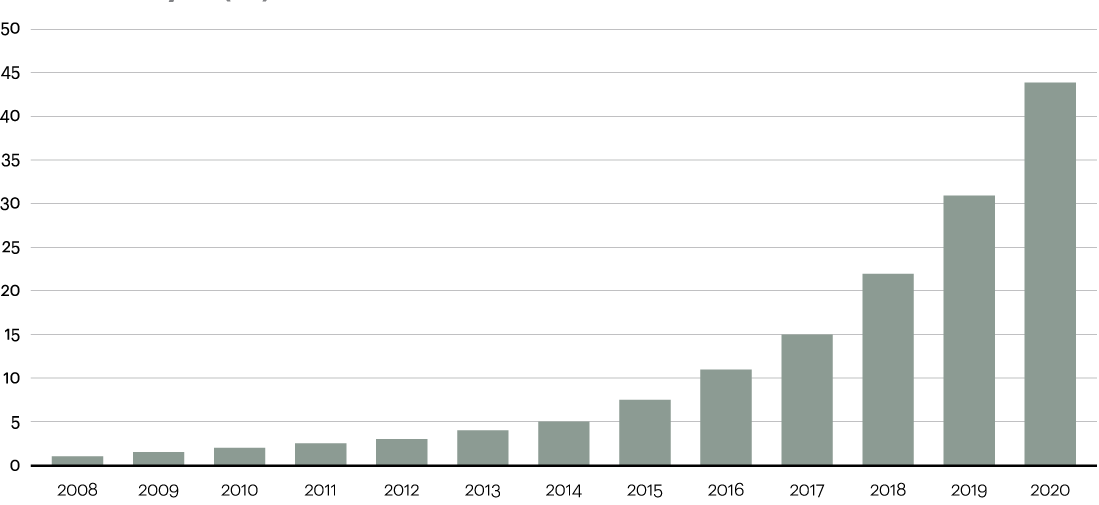
\includegraphics[width=14cm]{./images/Data.png}
	       	\caption{Evolución histórica del número de Zeta Bytes de información almacenados y predicción para los próximos años \cite{zeta-bytes}.} 
	       	\label{fig:zeta-bytes}
	 \end{figure}

	En resumen, a pesar de la evolución de los computadores en todas sus facetas, la cantidad de datos e información a procesar y almacenar crece incluso a mayor velocidad. Por ejemplo, encontramos empresas como Facebook y Google cuyos usuarios generan una gran cantidad de datos diariamente. Estos datos deben ser tratados en tiempo real para poder mantener los sistemas de recomendaciones asociados. En estos casos se requieren servidores de altas prestaciones para poder tratar tal cantidad de datos en un tiempo razonable. Estos conjuntos de datos adquieren el calificativo ``masivos''. El desarrollo de nuevas tecnologías, algoritmos y herramientas para tratar de forma eficiente conjuntos de datos masivos es lo que se conoce como Big Data \cite{big-data-herrera}.
	
	En este trabajo presentamos una introducción a Big Data y a las diferentes herramientas software existentes, destacando el papel de la ingeniería de servidores en este contexto. En particular, incidimos en la importancia del desarrollo de nuevos benchmarks que permitan evaluar las tecnologías de Big Data de forma clara y objetiva.

	El resto del texto se organiza como sigue. La Sección \ref{sec:big-data} contiene una descripción del concepto de Big Data. En la Sección \ref{sec:map-reduce} introducimos el paradigma de programación map reduce y la tecnología libre que lo implementa, denominada Hadoop. En la Sección \ref{sec:spark-flink} describimos las nuevas tecnologías que han surgido para cohesionar la filosofía map reduce con el procesamiento iterativo. Estas se denominan Spark y Flink. En la Sección \ref{sec:tpcx-hs} explicamos uno de los benchmarks existentes para las tecnologías Big Data, denominado TPCx-HS. Por último, en la Sección \ref{sec:conclusion} presentamos las conclusiones obtenidas.

\section{Big Data} \label{sec:big-data}
	
	En la Sección \ref{sec:introduction} hemos incidido en la rápida evolución que han sufrido los computadores. Sin embargo, en muchas aplicaciones encontramos conjuntos de datos que ponen a prueba a los ordenadores más ponentes. Estos conjuntos de datos se denominan masivos. El tratamiento de datos masivos tiene dos problemas claros. El primero de ellos es la memoria. Necesitamos computadores con suficiente memoria principal para procesar de forma eficiente un gran flujo de datos. El segundo problema es la capacidad de cómputo necesaria para aplicar algoritmos sobre estos conjuntos de datos. 
	
	Big Data engloba el tratamiento de datos masivos desde el punto de vista tecnológico y algorítmico. En palabras de Michael J. Franklin, profesor de informática en la universidad de Berkley \cite{bd-definition}:
	
	\textit{``Un problema sobre datos entra en el ámbito de Big Data cuando la aplicación de las actuales tecnologías no permite al usuario obtener soluciones  rápidas, efectivas en costo y de calidad''}

	Por tanto, Big Data es un concepto relativo a la situación tecnológica de la sociedad. Lo que hoy es Big Data puede no serlo dentro de varios años. Esto asegura que Big Data será un tema recurrente de la literatura especializada. La resolución de problemas de Big Data no cierra su desarrollo sino que abre nuevos retos, siempre habrá un conjunto de datos lo suficientemente grande como para poner a prueba los últimos logros del estado del arte.

	Los problemas que entran en el ámbito de Big Data surgen de manera natural en el mundo actual. En palabras de Francisco Herrera triguero, investigador de la Universidad de Granada  \cite{big-data-herrera}:
	
	\textit{``Vivimos en la era de la información. El progreso y la innovación no se ve obstaculizado por la capacidad de recopilar datos sino por la capacidad de gestionar, analizar, sintetizar y descubrir el conocimiento subyacente en dichos datos. Este es el reto de las tecnologías de Big Data.''}
	
	A veces se utiliza el término Big Data para referirse meramente a conjuntos de datos masivos. Sin embargo, los problemas de Big Data constan de múltiples características que los hacen todavía más complejos. En la literatura especializada estas características se denominan las 3 V's de Big Data \cite{big-data}:

	\begin{itemize}
		\item \textbf{Volumen.} El tamaño de los conjuntos de datos a procesar es cada vez mayor, por ejemplo, facebook procesa cada día 500 TB de información. Este volumen de datos requiere tecnologías específicas para que los servidores de altas prestaciones puedan manejar la información con éxito.
		\item \textbf{Velocidad.} Necesitamos herramientas que permitan procesar y analizar conjuntos de datos masivos en poco tiempo. Además, es habitual que el procesamiento de los datos deba ser incluso en tiempo real, esto es, los datos llegan al sistema de forma continua y este debe agregar la información de los mismos.
		\item \textbf{Variedad.} Los datos a tratar provienen de una gran variedad de fuentes. Por tanto, las herramientas Big Data deben permitir procesar a la vez datos de diferentes características y tamaños. Es más, habitualmente encontramos datos de tres tipos: estructurados, semi estructurados y sin estructurar. Los datos estructurados son sencillos de clasificar. Sin embargo, los datos sin estructurar son aleatorios y difíciles de analizar. Por su parte, los datos semi estructurados requieren técnicas avanzadas para poder clasificarlos correctamente.
	\end{itemize}

	Algunos autores han extendido la definición hasta utilizar un total de 9 V's: veracidad, valor, viabilidad y visualización entre otras \cite{understanding-big-data}. De esta forma se destacan diferentes aspectos del tratamiento de conjuntos de datos masivos como mantener y analizar la veracidad de los datos y poner en valor el conocimiento subyacente.

	El término Big Data ha tomado peso en el ámbito empresarial. Actualmente forma parte del área de conocimiento que se denomina inteligencia de negocio (business intelligence) \cite{business-intelligence}. La inteligencia de negocio cubre aquellos problemas relacionados con datos que se resuelven en organizaciones empresariales. Las empresas almacenan información de sus clientes y de toda la actividad realizada. Esta información contiene conocimiento que es valioso para determinar estrategias de negocio. Podemos decir que el análisis de datos es crucial para que las decisiones tomadas en la empresa sean efectivas. 

	También podemos considerar Big Data como parte del área denominada ciencia de datos \cite{data-science}. Esta es una temática emergente que aglutina todas las áreas científicas que se encargan del tratamiento de los datos y de la extracción de conocimiento de los mismos. En este contexto, algunos autores denominan Big Data Analytics a la aplicación de Big Data al análisis de datos \cite{big-data-trends}. 

%-----------------------------------------------------------------------------------------------------
%	SECCIÓN 2
%-----------------------------------------------------------------------------------------------------

\section{Map Reduce. Hadoop} \label{sec:map-reduce}


	\subsection{Servidores de altas prestaciones. Sistemas de archivos distribuidos}

		En la Sección \ref{sec:big-data} destacábamos dos problemas del tratamiento de conjuntos de datos masivos: el conjunto de datos puede no caber en memoria principal y se necesita una gran capacidad de cómputo para ejecutar algoritmos sobre este. La solución a este problema suele ser utilizar servidores de altas prestaciones con procesamiento en paralelo y distribuido.
	
		Los servidores de altas prestaciones (alguna descripción). .... 
		
		Los servidores contendrán ingentes cantidades de información de vital importancia. Por tanto, se necesita almacenar la información en un sistema de archivo tolerante a errores. Esto es, si un nodo o disco duro del servidor se estropea, no se pueden perder datos ni provocar una caída del servidor. En esta situación se encontró Google a principios de este siglo cuando desarrolló Google File System, GFS, que fue presentado oficialmente en 2003 \cite{gfs}. Este es un sistema de archivos escalable y distribuido que utilizan para aplicaciones distribuidas que requieran conjuntos de datos masivos. El sistema proporciona tolerancia ante fallos de forma automática y administra de forma eficiente grandes conjuntos de datos en el servidor, no necesitando que este sea especialmente caro. Además, proporciona escalabilidad en el sentido de que se pueden añadir o eliminar nodos o discos duros sin problemas. De esta forma, se consigue un correcto almacenamiento de los datos en el servidor.
		
		Google File System es un software privado. Basándose en las ideas de este, la fundación Apache ha desarrollado HDFS (Hadoop Distributed File System) \cite{hdfs}.

	\subsection{Map Reduce}


		Además de un sistema de archivos distribuido que asegure un correcto almacenamiento de la información en el servidor, se necesitan herramientas y librerías que permitan programar algoritmos paralelos y distribuidos. Las librerías OPEN MP y MPI (referencias) son muy conocidas. OPEN MP permite paralelizar cálculos vectoriales. Por su parte, MPI se basa en el paso de mensajes entre hebras como mecanismo para realizar implementaciones distribuidas. Estas librerías operan a bajo nivel y funcionan principalmente con lenguajes de programación como c y c++. 
		
		La implementación de un algoritmo distribuido utilizando estas librerías es muy costosa. El programador debe indicar expresamente el tratamiento distribuidos de los datos y cómo se paralelizan los cómputos. Además, tiene que crear las hebras asociadas y encargarse de que el sistema funcione correctamente. Nótese que si durante la ejecución el algoritmo un nodo se estropea, entonces la implementación puede dejar de funcionar a no ser que el programador le haya dedicado mucho tiempo para conseguir que sea tolerante ante fallos. Es más, si uno implementa varios algoritmos distribuidos esencialmente se está implementando el mismo tipo de paralelización una y otra vez.
	
		Ante esta situación en Google se dieron cuenta de la necesidad de desarrollar un nuevo paradigma de programación distribuida. Este debía proporcionar una interfaz para implementar algoritmos distribuidos de forma simple y eficiente sin tener que centrarse en cuestiones de bajo nivel. La distribución de los datos en los nodos y la tolerancia ante los fallos serían llevadas a cabo por el propio lenguaje de programación de manera que el programador solamente tiene que desarrollar el algoritmo en cuestión. Gracias a esta idea surge el paradigma de programación Map Reduce, que Google hace público en 2008 \cite{map-reduce1, map-reduce2, map-reduce3}.
	
		Map Reduce se basa en un proceso de abstracción a la hora de implementar algoritmos distribuidos. Los creadores de este paradigma se basaron en las funciones map y reduce que suelen estar presentes como primitivas en múltiples lenguajes de programación funcional. Un algoritmo se define como sigue. La entrada y la salida del algoritmo se conciben como dos listas de parejas clave / valor que pueden no tener los mismos tipos. El programador debe proporcionar el código de las funciones map y reduce.
		
		\begin{itemize}
			\item La función \textbf{map} toma como entrada una pareja clave / valor y produce un conjunto intermedio de parejas. Tras la ejecución de todos los maps, el sistema filtra los conjuntos intermedios de parejas obtenidos de manera que a cada posible clave se le asigna un conjuntos con todos los valores que tenía asociados como pareja.
			\item La función \textbf{reduce} toma una clave y un conjunto de valores asociados a la clave. Estos valores se mezclan, devolviendo al final cero o más parejas con la clave y los valores obtenidos tras la mezcla. El conjunto de valores que se proporciona como argumento a reduce se representa en la implementación mediante un iterador. De esta forma se puede trabajar con listas de valores tan grandes que no quepan en memoria principal.
		\end{itemize}  
		
		Para ejemplificar el funcionamiento de Map Reduce es habitual explicar cómo se puede contar el número de ocurrencias de cada una de las palabras de un texto. 
		
		\begin{algorithm}
			\caption{Algoritmo para contar el número de ocurrencias de cada una de las palabras de un texto en map reduce.}
			\label{alg:map}
			\begin{algorithmic}
				\REQUIRE Pareja (String key, String value) donde la clave representa el nombre del documento y el valor el contenido del documento.
				\FOR{\textbf{each word} $w$ \textbf{ in } $value$}
				\STATE EmitIntermediate(w, "1")
				\ENDFOR
			\end{algorithmic}

			\begin{algorithmic}
				\REQUIRE Pareja (String key, Iterator values) donde la clave consiste en una palabra del documento mientras que el iterador proporciona el número de veces que se ha encontrado la palabra en cada map.
				\STATE result = 0
				\FOR{each value $v$ in  $values$}
				\STATE result += ParseInt(v);
				\ENDFOR
				\STATE Emit(AsString(result));
			\end{algorithmic}
		\end{algorithm}
		



		Por tanto, se requieren tecnologías que manejen grandes conjuntos de datos de forma eficiente y a alto nivel, permitiendo que la implementación sea independiente del hardware a utilizar.

		Supóngase que una empresa compra un servidor en el cual ejecuta un algoritmo distribuido con eficiencia $\theta(n^2)$ sobre conjuntos de datos masivos. En el momento en el que se compra el hardware consiguen ejecutar el algoritmo en 8 horas, obteniendo resultados en el mismo día. Sin embargo, siguiendo la tendencia mostrada en la Figura \ref{fig:zeta-bytes}, es probable que al año el conjunto de datos a utilizar se duplique en tamaño dentro de un año. En tal caso el servidor puede tener problemas desde el punto de vista de la memoria y el flujo de datos. Es habitual que el hardware tenga cuellos de botella que provoquen que determinadas operaciones relacionadas con la memoria lleven mucho tiempo.  Por otro lado, el algoritmo tardará de todas formas 4 veces más en ejecutarse al ser cuadrático. Por tanto, la ejecución pasará a durar 32 horas, no pudiendo obtener resultados en un mismo día. 
		
		El ejemplo anterior muestra un problema de escalabilidad inherente a Big Data. Aunque esta claro que el procesamiento distribuido es la solución, el crecimiento de los conjuntos de datos hace que el hardware se quede obsoleto en poco tiempo. Una solución puede ser actualizarlo cada año. Sin embargo, una empresa no puede permitirse renovar el hardware anualmente pues esto supondría un aumento de costes, consumo eléctrico, mantenimiento y, además, requiere una gran cantidad de espacio. Otra solución consiste en reformular el algoritmo en cuestión, mejorando su eficiencia y escalabilidad.
		
		En cualquier caso, la solución que se tome implicará un gran trabajo para adaptar el software existente al nuevo hardware o para implementar nuevos algoritmos distribuidos. Cada nueva implementación conlleva multitud de líneas de código para manejar el conjunto de datos y realizar los cómputos distribuidos. Además, la implementación debe conseguir que el sistema sea tolerante ante fallos, esto es, si un nodo se estropea, entonces el sistema debe no perder la información y reasignar el trabajo del nodo a otro.

	\subsection{Hadoop}

%-----------------------------------------------------------------------------------------------------
%	SECCIÓN 3
%-----------------------------------------------------------------------------------------------------

\section{Spark y Flink} \label{sec:spark-flink}


%-----------------------------------------------------------------------------------------------------
%	SECCIÓN 4
%-----------------------------------------------------------------------------------------------------

\section{Benchmarks: TPCx-HS} \label{sec:tpcx-hs}

	La variedad de computadores es bastante heterogénea. Cada uno realiza de forma eficiente un determinado conjunto de operaciones a consta de presentar peores resultados en otros factores. Por tanto, la comparación entre diferentes modelos de computadores es compleja. Consecuentemente, se han creado benchmarks con el objetivo de aportar elementos de juicio con los que se discernir entre el uso de un computador u otro para una determinada aplicación. Habitualmente el benchmarking se define como la obtención de información útil mediante pruebas empíricas que ayude a una organización a mejorar sus procesos \cite{benchmarking}. Sin embargo, el benchmarking de computadores es un proceso costoso computacionalmente. Gasta tanto energía como mucho tiempo de cómputo. Por tanto, se ha de reservar para cuestiones sean importantes y no para evaluar tareas simples \cite{desv-bench}.
	
	Una técnica utilizada para ver qué sistema nos da más prestaciones son los benchmarks, uno de ellos es TPC. TPC es una organización sin ánimo de lucro que estudia el proceso de transacción y los benchmarks para las bases de datos. El término transacción se suele atribuir a aspectos bancarios, pero si pensamos en este concepto como una función que tienen los ordenadores, una transacción puede ser un conjunto de operaciones que incluyen lectura y escritura en disco, llamadas a funciones del sistema operativo, o cualquier forma de transferencia de datos de un sistema a otro. Este es el ámbito en el que se mueve TPC, que produce benchmarks que miden el proceso de transacción y el rendimiento de las bases de datos en términos de: dados un sistema y una base de datos, ¿cuántas transacciones pueden hacer por unidad de tiempo?\cite{intro-tpc}
	
	TPCx-HS se desarrolló para proveer de un rendimiento fiable, rendimiento relación precio, disponibilidad y, opcionalmente, datos de consumo de energía de los sistemas de Big Data. TPCx-HS fue el primer benchmark objetivo que permitía medir tanto hardware como software, como el Hadoop Runtime. \cite{info-tpc}
	
	\subsection{Carga de trabajo de TPCx-HS}
	
		La carga de trabajo de TPCx-HS consiste en los siguientes módulos \cite{tpcxhs}:
		
		\begin{itemize}
			\item HSGen: es un programa que genera los datos según factor de escala, que suele estar entre un 1TB y 10000TB(se denota TB como terabytes).
			\item HSDataCheck: es un programa que comprueba el cumplimiento del conjunto de datos.
			\item HSSort: es un programa que ordena los datos según un orden total.
			\item HSValidate: es un programa que valida la salida, es decir, los resultados obtenidos.
		\end{itemize}
	
	\subsection{Fases de ejecución del benchmark}
	
		Una ejecución válida consiste en cinco fases separadas que corren secuencialmente. Estas fases no se solapan en su ejecución, es decir, el comienzo de la fase 2 no puede darse hasta que la fase 1 esté completa. Para que comience cada fase se necesita de un script llamado <TPCx-HS-master> que es el que inicia cada fase y que puede ser ejecutado desde cualquier nodo del sistema que se está bajo test \cite{tpcxhs}.
		
		Las fases de ejecución son las siguientes:
		
		\begin{itemize}
			\item Fase 1: se generan los datos de entrada usando HSGen. Se han de copiar en un soporte duradero y hacer la copia replicada en tres discos (llamado \textit{"3-ways replication"}), que suelen ser el principal, el secundario y uno de respaldo\cite{replication}.
			\item Fase 2: se verifica la validez del conjunto de datos usando HSDataCheck. El programa sirve para verificar la cardinalidad, tamaño y el factor de réplica de los datos generados. Si el programa reporta un fallo, entonces la ejecución no es válida y se deberá volver a empezar.
			\item Fase 3: se lanza el programa HSSort con el que se ordena los datos de entrada. Esta fase muestra los datos de entrada y los datos de salida (los datos ya ordenados). Al igual que en la fase 1, se han de copiar los datos en un soportde duradero y hacer el \textit{"3-ways replication"}.
			\item Fase 4: se comprueba la viabilidad del conjunto de datos usando HSDataCheck. El programa comprueba la cardinalidad de los datos, tamaño y el factor de replicación de los datos ordenados. Si el programa reporta un fallo, entonces la ejecución no es válida y se deberá volver a empezar.
			\item Fase 5: validación de los datos con HSValidate. Como su nombre indica, HSValidate comprueba que los datos de salida sean correctos y si reporta el fallo consisten en que el HSSort no generó el correcto orden de salida, la ejecución se considerará inválida.
		\end{itemize}
		
		El benchmark consiste en dos ejecuciones (ver la Figura \ref{fig:ejecucionesTPC}) y cada vez que se ejecuta una fase se ha de especificar el tiempo que ha llevado la ejecución. Entre la primera ejecución de las cinco fases y la segunda, hay una fase intermedia que sirve para limpiar el sistema, conocida como \textit{"file system cleanup"} y, lógicamente, no se permite ninguna actividad durante dicha fase. Una vez realizadas las dos ejecuciones se obtiene el tiempo total de ejecución que servirá para calcular datos en la fase de medición.
		
		\begin{figure}[h]
			\centering
			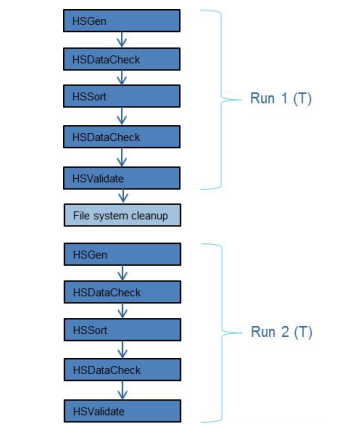
\includegraphics[width=5cm]{./images/executionsTPC.png}
			\caption{Gráfico de las ejecuciones de TPCx-HS} 
			\label{fig:ejecucionesTPC}
		\end{figure}
		
		Como consideraciones finales en la ejecución, el sistema bajo test no puede ser reconfigurado o cambiado durante o entre cualquiera de las fases de la ejecución ni tampoco entre la primera y la segunda ejecución. Cualquier cambio que se haga en el sistema se deberá realizar antes del comienzo de la fase 1 de la primera ejecución. El factor de escala usado en el conjunto de datos del test debe ser escogido del conjunto de factores de escala definido como sigue: 1TB, 3TB, 10TB, 30TB, 100TB, 300TB, 1000TB, 3000TB, 10000TB.
	
	\subsection{Medida del rendimiento}
	
		Para hacer el análisis de la medida del rendimiento, TPCx-HS define las siguientes medidas:
		
		\begin{itemize}
			\item HSph@SF: refleja la medida del rendimiento de TPCx-HS.
			\item \$/HSph@SF: es la medida del rendimiento-precio.
			\item Si se escoge la opción de \textit{"TPC-energy"}, la medida de la energía que hace TPCx-HS informa de la potencia por rendimiento. \\
		\end{itemize}
		
		La medida del rendimiento se representa con HSph@SF, que se mide con la siguiente expresión:
		
		$$ HSph@SF = \frac{SF}{T/3600} $$
		
		donde:
		\begin{itemize}
			\item SF es el factor de escala escogido.
			\item T es el tiempo total que se obtuvo al sumar el tiempo de las dos ejecuciones. \\
		\end{itemize}	
		
		La medida del rendimiento-precio se puede calcular con la siguiente fórmula:
		
		$$ \$/HSph@SF = \frac{P}{HSph@SF} $$
		
		donde P es el costo del sistema en el que se han hecho las ejecuciones.
		
		\subsection{Comparación de la medida}
		
		Un resultado dado por la ejecución de TPCx-HS sólo puede ser comparado con otro resultado que provenga de la ejecución de este benchmark y que tenga el mismo factor de escala. Otras consideraciones a tener en cuenta son:
		
		\begin{itemize}
			\item Los resultados producidos por test que tienen diferente factor de escala no son comparables, debido a los \textit{retos} computacionales encontrados en volúmenes de datos de distinto tamaño.
			\item Si los resultados medidos con diferentes factores de escalas aparecen impresos o en algún documento electrónico, entonces cada referencia que se haga a uno de estos resultados se ha de especificar claramente el factor de escala que se usó para obtener esos resultados. Si los resultados aparecen de forma gráfica, el factor de escala en el que se basó dicha medición se deberá poder discernir, por ejemplo usando una etiqueta en uno de los ejes.
		\end{itemize}
		
		
		Se presenta a continuación una tabla con los resultados para algunas compañías donde se puede ver el factor de escala usado, el sistema y los resultados obtenidos tras la ejecución del benchmark.
		
		\begin{figure}[H]
			\centering
			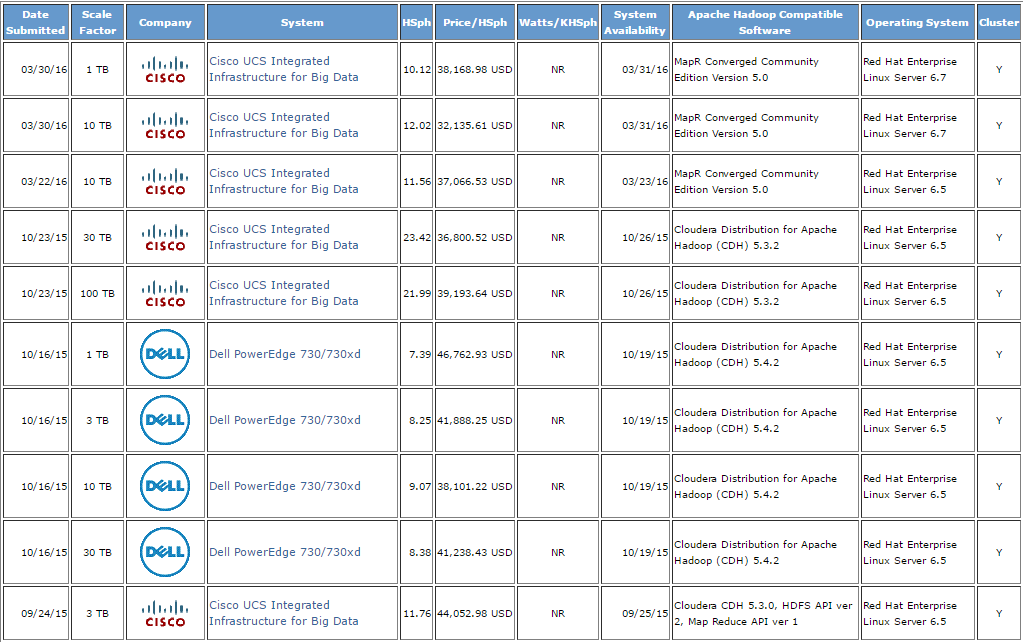
\includegraphics[width=15cm]{./images/examples.png}
			\caption{Tabla de resultados obtenidos con TPCx-HS \cite{ejemplos}.} 
			\label{fig:ejemplo}
		\end{figure}

%-----------------------------------------------------------------------------------------------------
%	SECCIÓN 5: CONCLUSIÓN
%-----------------------------------------------------------------------------------------------------

\section{Conclusión} \label{sec:conclusion}

	Podemos decir que Big Data es un área que aúna tanto la ingeniería del software como la ingeniería de servidores y la ciencia de datos.

%-----------------------------------------------------------------------------------------------------
%	SECCIÓN X: REFERENCIAS
%-----------------------------------------------------------------------------------------------------

\printbibliography

\end{document}